\documentclass[]{article}

\usepackage[margin=1.2in]{geometry} 
\usepackage{amsmath}
\usepackage{color}
\usepackage{float}
\usepackage{graphicx}
\usepackage{graphicx}
\usepackage{hyperref}
\usepackage{listings}
\usepackage{listings}
\usepackage{parskip}
\usepackage{subfig}
\usepackage{url} 

\definecolor{lightgray}{rgb}{.9,.9,.9}
\definecolor{darkgray}{rgb}{.4,.4,.4}
\definecolor{purple}{rgb}{0.65, 0.12, 0.82}

\lstdefinelanguage{JavaScript}{
  keywords={typeof, new, true, false, catch, function, return, null, catch, switch, var, if, in, while, do, else, case, break},
  keywordstyle=\color{blue}\bfseries,
  ndkeywords={class, export, boolean, throw, implements, import, this},
  ndkeywordstyle=\color{darkgray}\bfseries,
  identifierstyle=\color{black},
  sensitive=false,
  comment=[l]{//},
  morecomment=[s]{/*}{*/},
  commentstyle=\color{purple}\ttfamily,
  stringstyle=\color{red}\ttfamily,
  morestring=[b]',
  morestring=[b]"
}

\lstset{
    basicstyle=\footnotesize\ttfamily,
    numbers=left
}

\begin{document}

\title{Globe Crime Visualization}
\author{Roy Portas - s4356084}
\date{\today}
\maketitle 

\begin{large}
    \begin{center}
        Final product available at \url{https://r-portas.github.io/crime-globe/}

        Source code available at \url{https://github.com/r-portas/crime-globe}
    \end{center}
\end{large}

\break

\section{Introduction}

Crime occurs all around the world and is caused by many factors.
Knowing crime rates of cities is useful for travellers planning journeys, thus it would be useful to provide a
method to visualize this.

The aim of this project is to create a web based visualization of global crime data.
This will be done through a 3D model of a globe with crime data superimposed on top of it.
Computer graphics will be utilized to draw this model in 3D and to make it look realistic.
The goal is to create a realistic looking world and lighting.

The visualization aims to be a easy to use tool for the general public to view crime trends around the world over time.
Thus for it to be accessible it was decided to build the project using Javascript and WebGL,
as this means anyone with a web browser can access the project.

\section{Methods}

\subsection{Acquiring Data and Domain Research}

Data was acquired from the website \url{https://knoema.com/atlas/topics/Crime-Statistics}.

Before building the web app, research was done on existing solutions, such as Google Earth and Marble.

From looking at existing solutions, some common functionality was found

\begin{itemize}
	\item Rotating the globe
	\item Zooming the globe
	\item High resolution texturing
	\item Lighting that emulates the sun and day/night cycles
\end{itemize}

From researching computer graphics methods, some additional concepts that can be applied include:

\begin{itemize}
	\item Using a bump map to simulate the mountains and valleys of the world
	\item Specular maps to make the water look reflective
\end{itemize}

\subsection{Designing the Object Hierarchy}

The object hierarchy allows us to define groups of objects to manage the transformations and rotations more easily.
It usually takes the form of a tree structure with leaf nodes being the smallest parts of the model.

The complete model will consist of the following elements:

\begin{itemize}
	\item The world
	\item The camera
	\item The sun (light source)
	\item The moon, which rotates around the world
	\item Crime heat maps, which are displaying on the world.
\end{itemize}

Thus the model can be representing in the following hierarchy:

\begin{figure}[H]
   \centering
   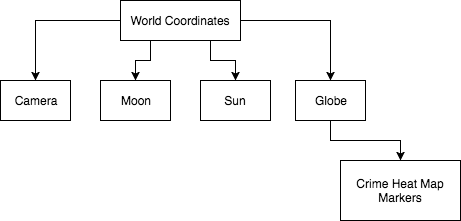
\includegraphics[width=0.5\linewidth]{images/object_hierachy}
   \caption{Object Hierarchy}
   \label{fig:object_hierarchy}
\end{figure}

\subsection{Version 1: Pure WebGL}

The initial prototype was created in pure WebGL, which is graphics library for web browsers with an API similar to OpenGL ES2.0.
The first step to creating the WebGL program is initialize WebGL and setup the shaders and buffers.
To start with a simple cube was created, the shape of the cube was defined as vertices.

\begin{lstlisting}[language=JavaScript]
const cubeVertexBuffer = gl.createBuffer();
gl.bindBuffer(gl.ARRAY_BUFFER, cubeVertexBuffer);
const vertices = [
    // Front face
    -1.0, -1.0,  1.0,
    1.0, -1.0,  1.0,
    1.0,  1.0,  1.0,
    -1.0,  1.0,  1.0,

    // Back face
    -1.0, -1.0, -1.0,
    -1.0,  1.0, -1.0,
    1.0,  1.0, -1.0,
    1.0, -1.0, -1.0,

    .... // Do for all faces
];

gl.bufferData(gl.ARRAY_BUFFER, new Float32Array(vertices), gl.STATIC_DRAW);

// We are using 3 dimensions
cubeVertexBuffer.itemSize = 3;
// We need 24 vertices to represent a cube
cubeVertexBuffer.numItems = 24;
\end{lstlisting}

This buffer contains all the points required to create a cube.
WebGL then takes this JavaScript and converts it into GLSL, which is ran on the GPU.

After defining the position vertices, the colour buffer was created, for this example
the colours was kept simple, a solid green colour for all the cube.

Once these buffers are setup, the next thing to do is to setup the shaders.
For this prototype two shaders where used, a fragment shader and a vertex shader.

The fragment shader in this case just sets up the GPU to use the correct data types for the rest of the code.
The vertex shader generates coordinates in the clipspace, which is used by the GPU to render the objects correctly.

Once these shaders were created two matrices were set up, one for the model view matrix, the other for the projection matrix.
The model view matrix transforms coordinates into view coordinates, which is used by the GPU to display the objects.
The projection matrix is used to used to manage the perspective of the scene.

\begin{figure}[H]
   \centering
   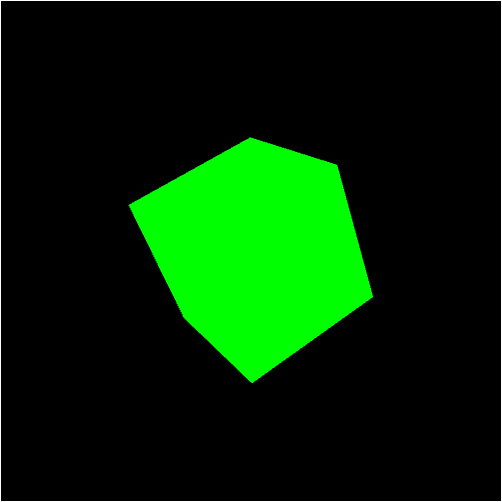
\includegraphics[width=0.5\linewidth]{images/webgl_cube}
   \caption{Simple WebGL Application}
   \label{fig:webgl_cube}
\end{figure}

Figure~\ref{fig:webgl_cube} shows the simple application running.
The program just shows a cube, without any lighting.
However the code to generate this cube was quite verbose, luckily there is a variety of Javascript frameworks which provide wrappers around the WebGL interface.

One such framework is ThreeJS, which provides a lot of helper functions to make creating programs easier.

\subsection{Version 2: ThreeJS}

As the project became more complex, it became hard to manage all the WebGL code.
Thus a third party library called ThreeJS was used.
ThreeJS provides a lot of useful helper functions to write WebGL applications more easily,
such support for animations, common geometries and lighting.

\subsubsection{Setting up the Scene}

ThreeJS provides some helper functions on top of WebGL to create scenes more easily.

For a simple application, a sphere was created in the center of the scene with a camera looking at it.
The projection matrix logic is abstracted into the camera, thus for a 3D application a PerspectiveCamera was used.
The PerspectiveCamera calculates the projection matrix for visible objects, which saves writing a lot of GSLS code.

The sphere was draw using a simple mesh that does not react to lighting changes and has a solid colour of blue.
The result is shown in Figure~\ref{fig:plainSphere}.

\begin{figure}[H]
   \centering
   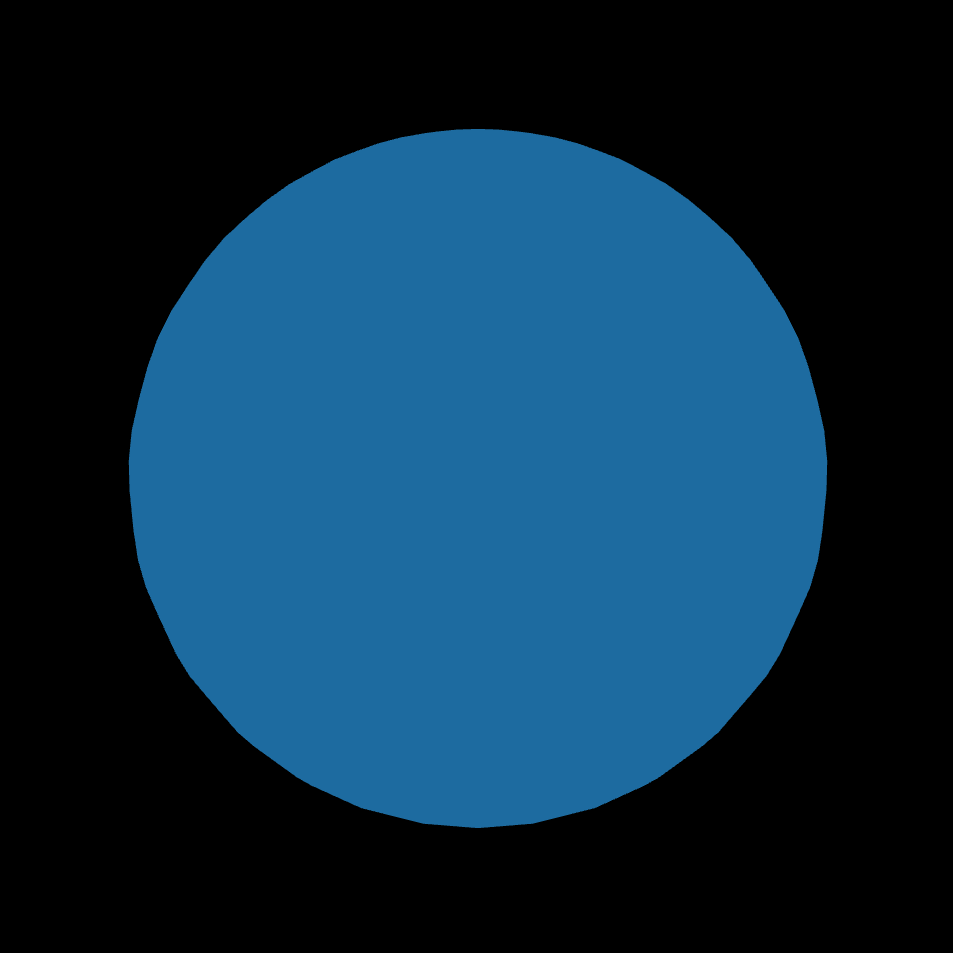
\includegraphics[width=0.5\linewidth]{images/plain_sphere}
   \caption{Plain Sphere}
   \label{fig:plainSphere}
\end{figure}

\subsubsection{Meshes and Shading}

The sphere looks plain without any lighting applied to it,
thus the type of mesh was changed to one that supports shading.

ThreeJS supports Physically Based Rendering, which simulates natural light iterations with real world materials\cite{physically_based_rendering}.
PBR in ThreeJS uses image based lighting that allows objects in the scene to pick up surrounding colours from the environment.

More specifically ThreeJS uses the Metallic Roughness style of PBR.
This method uses two maps, one for roughness and one of metalness.
Roughness is similar to conventional specular maps,
however is better optimized for real time rendering\cite{meshstandardmaterial_2017}.
Metalness defines how metallic an object is,
which affects the way light is reflected from the object.

Adding PBF to the simple sphere model allows light to be reflected from it as well as adding a shadow to the sphere,
which can be seen in Figure~\ref{fig:pbf_sphere}.

\begin{figure}[H]
   \centering
   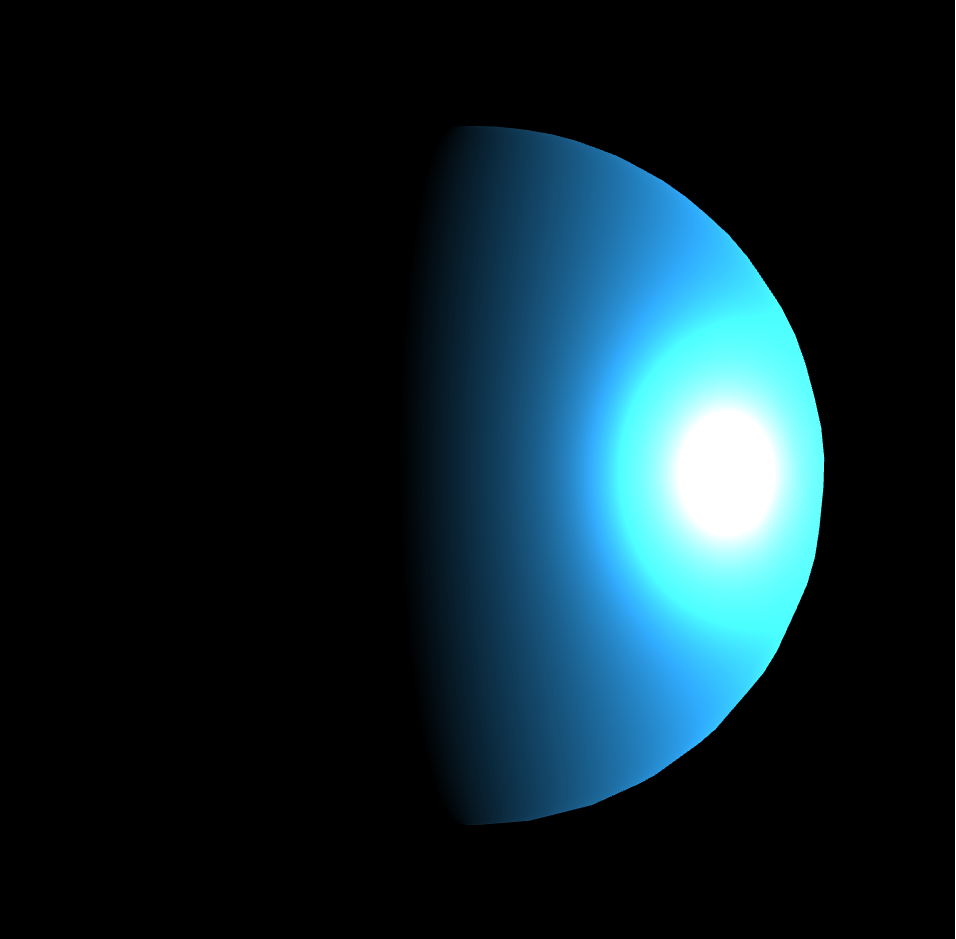
\includegraphics[width=0.5\linewidth]{images/pbf_sphere}
   \caption{PBF Sphere}
   \label{fig:pbf_sphere}
\end{figure}

\subsubsection{Texturing and Maps}

The next step is to apply the texture to the sphere.
The texture was downloaded from \url{http://www.shadedrelief.com/natural3/index.html},
which offers high resolution globe images for free.

Texturing the sphere in ThreeJS is easy, it just requires loading the image then applying the texture to the object.
The final result can be seen in Figure~\ref{fig:textured_sphere}.

\begin{figure}[H]
   \centering
   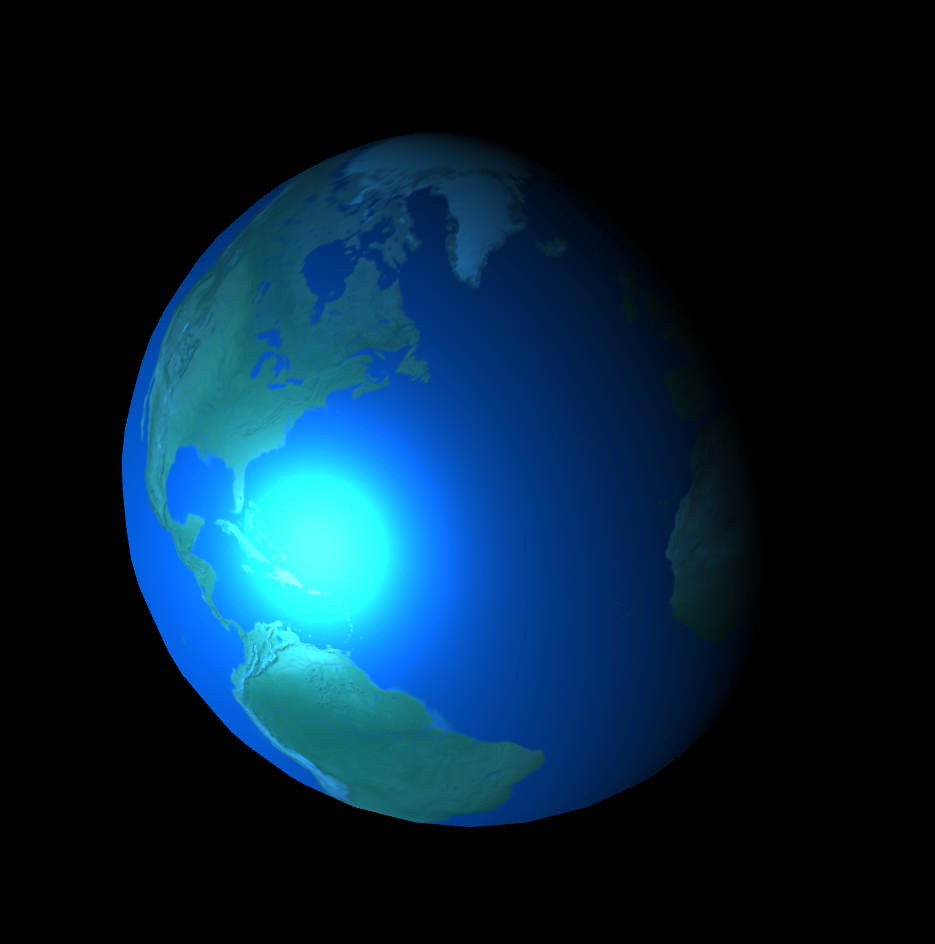
\includegraphics[width=0.5\linewidth]{images/textured_sphere}
   \caption{Textured Sphere}
   \label{fig:textured_sphere}
\end{figure}

At the moment the lighting system is extracting the blue colour from the ocean to give the light a blueish hue.
This will be corrected when the lighting is improved.

Next a bumpmap can be applied to the globe to simulate mountains and valleys on the earth.
Bump maps do not modify the actual surface, instead the surface normal is is modified as if the surface has been moved.
This results in a more real looking world.
The bump map looks similar to a standard texture, but is in greyscale with darker colours signifying a greater height and lighter colours representing a lower height.
ThreeJS will use the Phong reflection model\cite{meshstandardmaterial_2017} to display the bump map onto the globe.


The bump maps were downloaded from the same site that provided the earth maps.

\begin{figure}[H]
    \centering
    \subfloat[0.05 scale]{{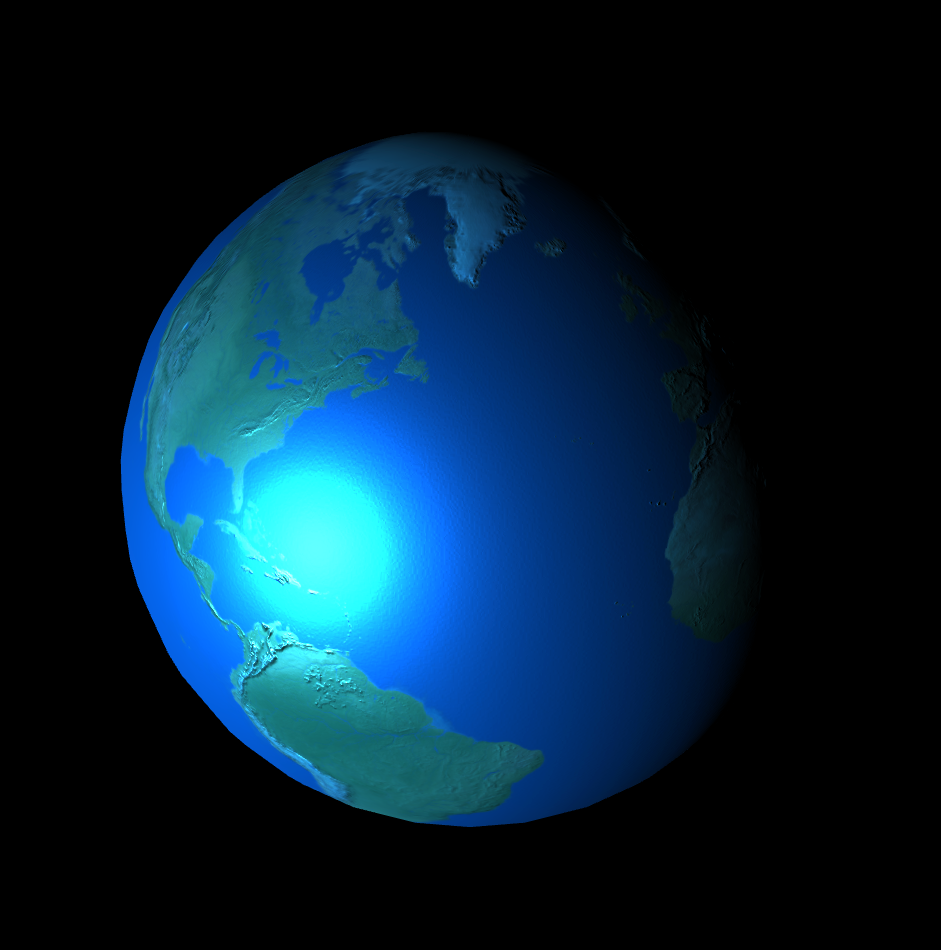
\includegraphics[width=0.3\linewidth]{images/bumpmap_0_05}}}%
    \qquad
    \subfloat[0.2 scale]{{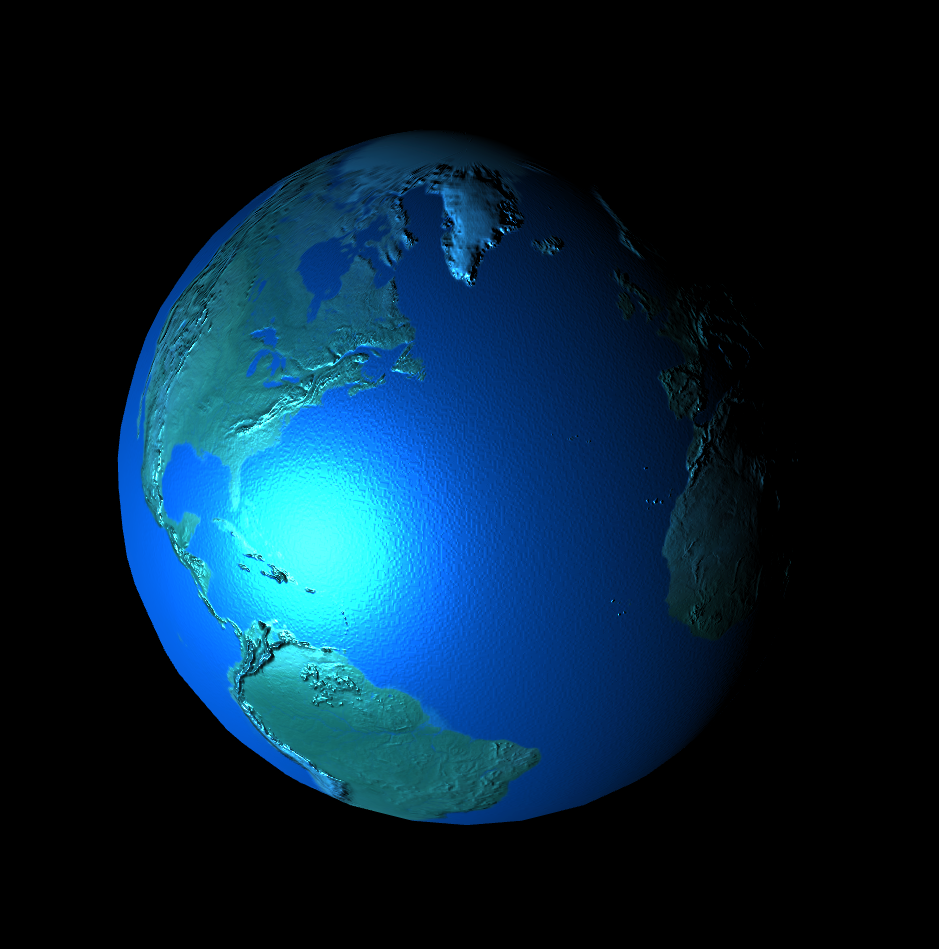
\includegraphics[width=0.3\linewidth]{images/bumpmap_0_2}}}%
    \qquad
    \subfloat[1 scale]{{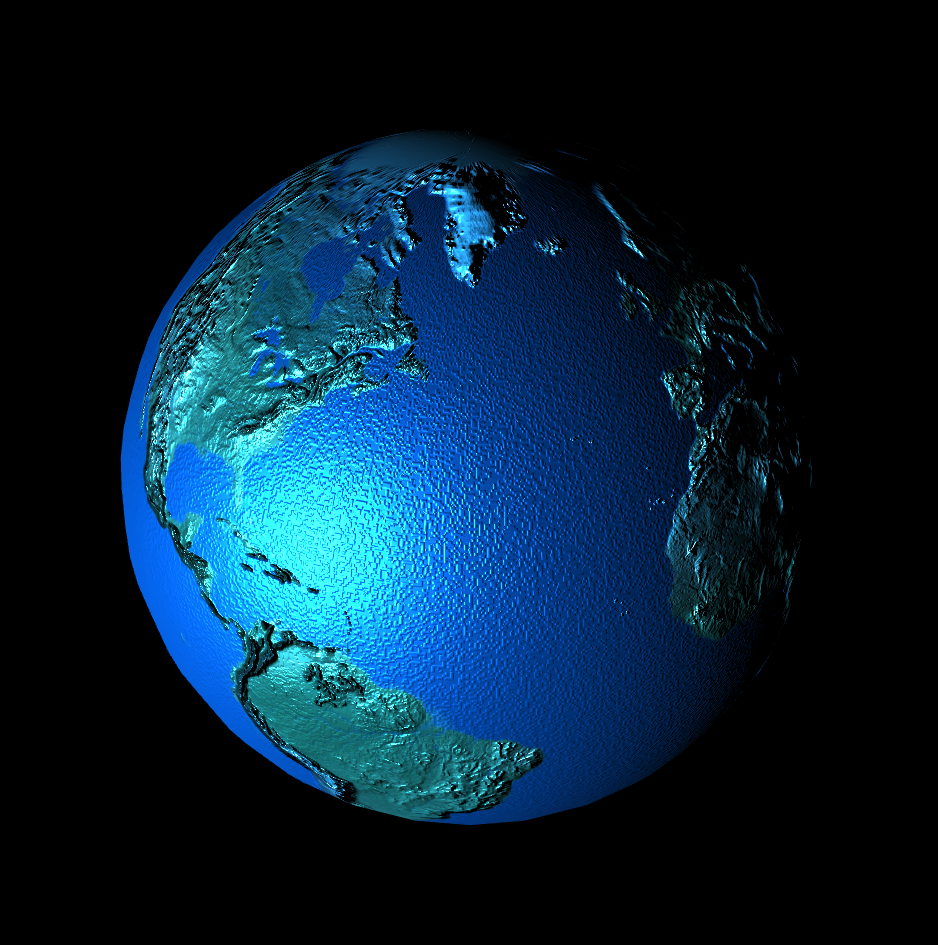
\includegraphics[width=0.3\linewidth]{images/bumpmap_1}}}%
    \qquad
    \caption{Bump Map Comparison}
    \label{fig:bumpmap}
\end{figure}

Figure~\ref{fig:bumpmap} shows different values for scales for the bump maps.
Choosing the right scale is important for realism, as a too high value will over exaggerate small displacements,
such as ocean sea levels.
This effect is shown in the third image.
However choosing a too small value will not give the desired effect and result in a flat looking planet.

The second scale was chosen, as it provided a nice looking result.

\subsubsection{Lighting and Specular Maps}

The next step is to improve lighting to make the scene look more realistic.
To do this two lights will be used, one to represent the sun and another that follows the camera.

The sun light will light up the Earth and simulate the earth revolving around the sun.
It will be the brightest light in the scene.

This will be implemented as a directional light that points at the Earth,
as this is more efficient than something like a point light, that will reflect light in all directions.

The second light is a smaller light that follows the camera,
allowing the globe to be visible when the sun is behind the Earth.
This light will also be implemented as a directional light and will follow the camera around the scene.
The target of this light will also be the Earth.

After lighting the specular map was implemented.
Specular maps control the reflectiveness of an object.
It works similar to a bump map, being a grey scale image with white being reflective
and black being non reflective.
This allows an object to have areas of more reflectiveness,
which in our case will be the ocean.
Land will be represented as less reflective.
This makes the globe seem more realistic.

\subsubsection{Orbiting Moon}

The next step is to draw an orbitting moon around the Earth.
This is similar to drawing the Earth, but also requires the moon to orbit the earth.
The exact orbit will follow a simple equation, outlined below:

\begin{align*}
    x &= n \times sin(i)\\
    y &= n \times cos(i)
\end{align*}

Where $n$ is the distance from the center of the Earth to the moon and $i$ is the time.

After implementing this the next step was to set up the shadows of the moon.
This requires three parts:

\begin{itemize}
    \item The renderer - Does all the computation
    \item The Sun - Which casts shadows
    \item The moon and Earth - Which receives the lights and shadows
\end{itemize}

\subsubsection{Displaying Crime Data}

The next step is to display the crime data on the globe.
This data was acquired from Knoema, available here \url{https://knoema.com/CMI2017/crime-index-by-country-2017}.
The data was given in a CSV format with city name, and crime value as columns.
The crime value is a index of how much crime happens in the city, which ranges between
0 for no crime and 100 for the most crime activity.

The first step was to convert the city names to longitude and latitude values,
this was done using the Google Geocoding API.

Below is a sample HTTP request for getting the longitude and latitude from the location.

\begin{verbatim}
curl https://maps.googleapis.com/maps/api/geocode/json?address=Yerevan&key=$GOOGLE_API_KEY
\end{verbatim}

This was used in a python program to get the latitudes and longitudes for all cities in the dataset.
The coordinates were than mapped to the city name and the crime rate for the city.
The final result was exported as a json file that could be easily imported into the application.

The next step was to convert the coordinates into something useable by the program.
This required a bit of maths and angle calculations.

\begin{lstlisting}[language=JavaScript]
    convertToSphere(coords) {
      const phi = (90 - coords[0]) * (Math.PI / 180);
      const theta = (coords[1] + 180) * (Math.PI / 180);
      const offset = 300;

      const x = -((this.globeRadius + offset) * Math.sin(phi) * Math.cos(theta));
      const y = ((this.globeRadius + offset) * Math.cos(phi));
      const z = ((this.globeRadius + offset) * Math.sin(phi) * Math.sin(theta));

      return new three.Vector3(x, y, z);
    },
\end{lstlisting}

\begin{figure}[H]
   \centering
   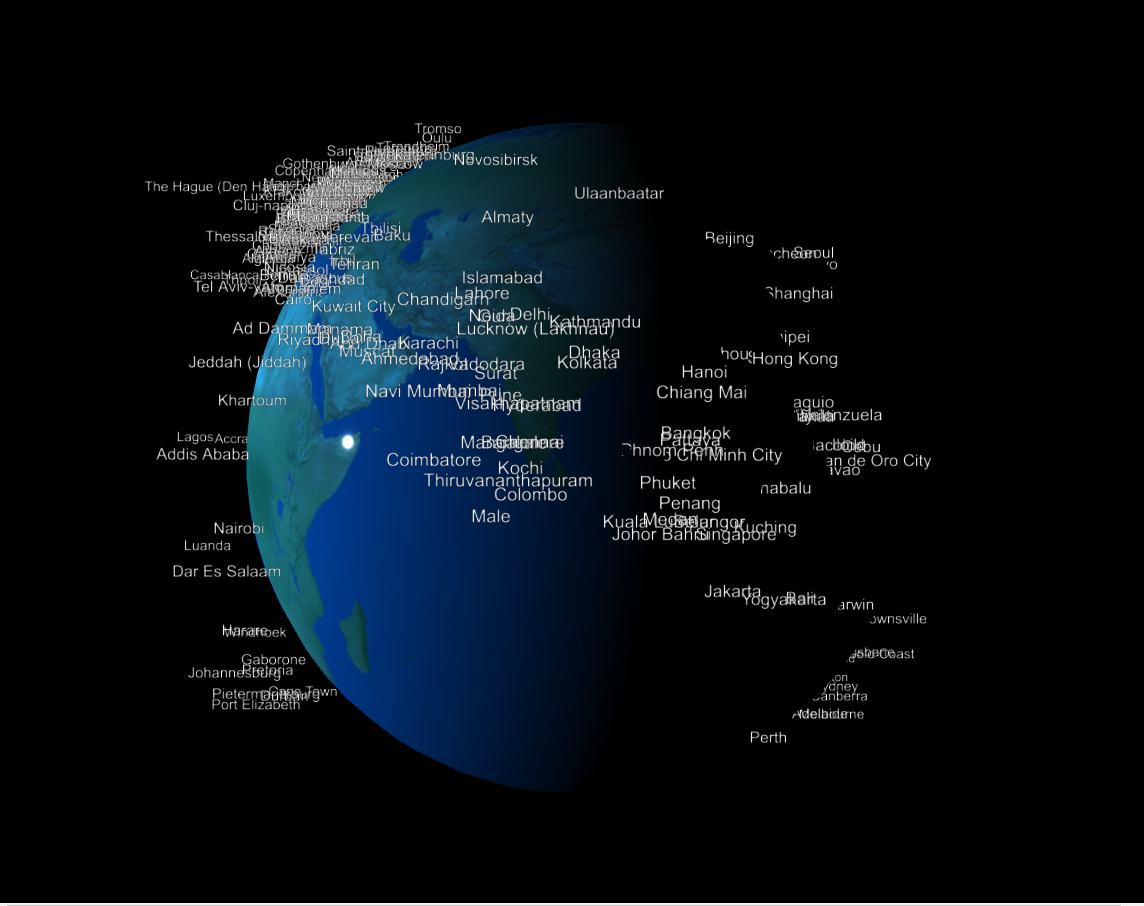
\includegraphics[width=0.8\linewidth]{images/city_labels}
   \caption{Cities with Labels}
   \label{fig:city_labels}
\end{figure}

Figure~\ref{fig:city_labels} shows an overlay of city names on the globe.
This was done using the coordinates from the convertToSphere function and just plotting a label onto the map.

The next step was to draw a representation of crime at each of these coordinates,
this was done by drawing a sphere over the location of the crime.
The radius of the sphere is determined by the amount of crime in the area,
with more crime having a larger sphere.

The final step was to change the colour of the sphere depending on the amount of crime.
This was simply done by changing the red value depending on the crime rate of the area.

\begin{figure}[H]
   \centering
   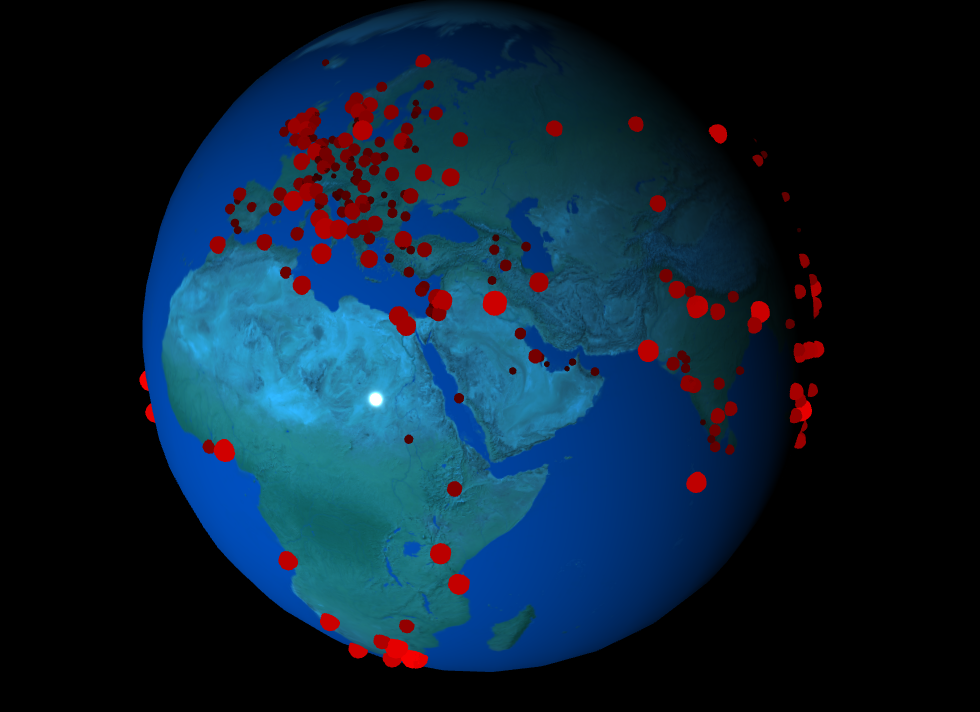
\includegraphics[width=0.8\linewidth]{images/crime_spheres}
   \caption{Crimes Displayed as Spheres}
   \label{fig:crime_spheres}
\end{figure}

\subsection{User Interaction and Camera}

The final step was to implement interaction with the globe, 
to allow the user to rotate to see all the crime data.

This was done by rotating the camera around the globe,
as this required less computational effort then moving all the data points.

To do this camera was set to an initial vector of (100000, 0, 0),
then updated when the user moves the mouse.
This was done by using 2 angles, one for the x and y axis.
These angles were called Phi and Theta.
By changing these angles the camera will rotate around the earth.
The math behind it is very similar to the math used to convert longitude
and latitude coordinates to world coordinates.

The trick to doing this was to update the angles according to mouse movement.
The easiest way to do this was to calculate the mouse movement distance during
each drag and adding that onto the respective angle, depending on the direction of the drag.


\section{Results}

The final result is hosted at \url{https://r-portas.github.io/crime-globe/}.
Depending on internet connection speed the globe textures could take a while to download.

There is also a git repo hosted at \url{https://github.com/r-portas/crime-globe} which contains the
full commit history on the project and all source code.
Build instructions are also in the repo.

This project employed a lot of the computer graphics techniques covered through this course, outlined below.

\subsection{Texturing Models}

Texturing models was important for rendering a realistic looking version of the Earth.
For this project 3 textures were used, a texture map, bump map and specular map.
These provided a more realistic representation of the Earth.

\subsection{Lighting and Cameras}

Lighting and cameras played a large part in the end product.
The lighting is reflected on the planet, which makes a realistic looking ocean.

The main light in the scene is the Sun, which was created using a directional light.
This gave the effect of the sun rotating around the world to simulate a day and night cycle.

\subsection{Transformations}

Transformations were used to move the crime data points into the correct position around the globe.
Additionally transformations were used to move the camera and sun around the scene.

\section{Discussion}

Overall the construction of this simulation went well,
with all featured implemented as desired.
I gained experience using a variety of computer graphics techniques in WebGL,
such as 3D rendering, lighting, texturing and transformations.

One improvement for the project is improving the performance of the application.
This comes down to optimising the way the objects are drawn onto the canvas.
This current method involves a lot of drawing and then moving components, with
some object references becoming lost from the renderer at some points, which
caused a decrease in performance.

Another improvment is implementing time based data.
The dataset also contained data over time and it would be
interesting to allow the user to select the time period and see how global crime changes over time.
This could be done by redrawing the scene each time, but this was found to be too intensive.
Thus the code will have to be refactored to support updating of the data and then scale the size
of the crime areas, but this took too long so was excluded from the project.

Another improvement is providing more data to the user, maybe in the form of a label over each
data point so the user can see more detailed information about a particular city.
This is more of a user interface feature than a computer graphics task, but would 
provide value to the users.

\section{Conclusion}

The final version of the software is available at \url{https://r-portas.github.io/crime-globe/}.
The software is fully functional and runs on any modern browser.
The project has implemented many of the methods taught throughout the course
and proved to be a value learning experience in developing 3D equations.

There are some improvements that can be made, mostly around the optimization of the software 
such that it runs better on slower devices.
However overall the project achieves the purpose of providing an accessible visualization of crime data.

\break

\begin{large}
    \begin{center}
        Final product available at \url{https://r-portas.github.io/crime-globe/}

        Source code available at \url{https://github.com/r-portas/crime-globe}
    \end{center}
\end{large}

\bibliographystyle{abbrvurl}
\bibliography{bibliography}

\end{document}
